\documentclass[]{article}
\usepackage{lmodern}
\usepackage{amssymb,amsmath}
\usepackage{ifxetex,ifluatex}
\usepackage{fixltx2e} % provides \textsubscript
\ifnum 0\ifxetex 1\fi\ifluatex 1\fi=0 % if pdftex
  \usepackage[T1]{fontenc}
  \usepackage[utf8]{inputenc}
\else % if luatex or xelatex
  \ifxetex
    \usepackage{mathspec}
  \else
    \usepackage{fontspec}
  \fi
  \defaultfontfeatures{Ligatures=TeX,Scale=MatchLowercase}
\fi
% use upquote if available, for straight quotes in verbatim environments
\IfFileExists{upquote.sty}{\usepackage{upquote}}{}
% use microtype if available
\IfFileExists{microtype.sty}{%
\usepackage{microtype}
\UseMicrotypeSet[protrusion]{basicmath} % disable protrusion for tt fonts
}{}
\usepackage[margin=1in]{geometry}
\usepackage{hyperref}
\hypersetup{unicode=true,
            pdftitle={Homework 3},
            pdfauthor={Megha Pandit},
            pdfborder={0 0 0},
            breaklinks=true}
\urlstyle{same}  % don't use monospace font for urls
\usepackage{color}
\usepackage{fancyvrb}
\newcommand{\VerbBar}{|}
\newcommand{\VERB}{\Verb[commandchars=\\\{\}]}
\DefineVerbatimEnvironment{Highlighting}{Verbatim}{commandchars=\\\{\}}
% Add ',fontsize=\small' for more characters per line
\usepackage{framed}
\definecolor{shadecolor}{RGB}{248,248,248}
\newenvironment{Shaded}{\begin{snugshade}}{\end{snugshade}}
\newcommand{\KeywordTok}[1]{\textcolor[rgb]{0.13,0.29,0.53}{\textbf{#1}}}
\newcommand{\DataTypeTok}[1]{\textcolor[rgb]{0.13,0.29,0.53}{#1}}
\newcommand{\DecValTok}[1]{\textcolor[rgb]{0.00,0.00,0.81}{#1}}
\newcommand{\BaseNTok}[1]{\textcolor[rgb]{0.00,0.00,0.81}{#1}}
\newcommand{\FloatTok}[1]{\textcolor[rgb]{0.00,0.00,0.81}{#1}}
\newcommand{\ConstantTok}[1]{\textcolor[rgb]{0.00,0.00,0.00}{#1}}
\newcommand{\CharTok}[1]{\textcolor[rgb]{0.31,0.60,0.02}{#1}}
\newcommand{\SpecialCharTok}[1]{\textcolor[rgb]{0.00,0.00,0.00}{#1}}
\newcommand{\StringTok}[1]{\textcolor[rgb]{0.31,0.60,0.02}{#1}}
\newcommand{\VerbatimStringTok}[1]{\textcolor[rgb]{0.31,0.60,0.02}{#1}}
\newcommand{\SpecialStringTok}[1]{\textcolor[rgb]{0.31,0.60,0.02}{#1}}
\newcommand{\ImportTok}[1]{#1}
\newcommand{\CommentTok}[1]{\textcolor[rgb]{0.56,0.35,0.01}{\textit{#1}}}
\newcommand{\DocumentationTok}[1]{\textcolor[rgb]{0.56,0.35,0.01}{\textbf{\textit{#1}}}}
\newcommand{\AnnotationTok}[1]{\textcolor[rgb]{0.56,0.35,0.01}{\textbf{\textit{#1}}}}
\newcommand{\CommentVarTok}[1]{\textcolor[rgb]{0.56,0.35,0.01}{\textbf{\textit{#1}}}}
\newcommand{\OtherTok}[1]{\textcolor[rgb]{0.56,0.35,0.01}{#1}}
\newcommand{\FunctionTok}[1]{\textcolor[rgb]{0.00,0.00,0.00}{#1}}
\newcommand{\VariableTok}[1]{\textcolor[rgb]{0.00,0.00,0.00}{#1}}
\newcommand{\ControlFlowTok}[1]{\textcolor[rgb]{0.13,0.29,0.53}{\textbf{#1}}}
\newcommand{\OperatorTok}[1]{\textcolor[rgb]{0.81,0.36,0.00}{\textbf{#1}}}
\newcommand{\BuiltInTok}[1]{#1}
\newcommand{\ExtensionTok}[1]{#1}
\newcommand{\PreprocessorTok}[1]{\textcolor[rgb]{0.56,0.35,0.01}{\textit{#1}}}
\newcommand{\AttributeTok}[1]{\textcolor[rgb]{0.77,0.63,0.00}{#1}}
\newcommand{\RegionMarkerTok}[1]{#1}
\newcommand{\InformationTok}[1]{\textcolor[rgb]{0.56,0.35,0.01}{\textbf{\textit{#1}}}}
\newcommand{\WarningTok}[1]{\textcolor[rgb]{0.56,0.35,0.01}{\textbf{\textit{#1}}}}
\newcommand{\AlertTok}[1]{\textcolor[rgb]{0.94,0.16,0.16}{#1}}
\newcommand{\ErrorTok}[1]{\textcolor[rgb]{0.64,0.00,0.00}{\textbf{#1}}}
\newcommand{\NormalTok}[1]{#1}
\usepackage{graphicx,grffile}
\makeatletter
\def\maxwidth{\ifdim\Gin@nat@width>\linewidth\linewidth\else\Gin@nat@width\fi}
\def\maxheight{\ifdim\Gin@nat@height>\textheight\textheight\else\Gin@nat@height\fi}
\makeatother
% Scale images if necessary, so that they will not overflow the page
% margins by default, and it is still possible to overwrite the defaults
% using explicit options in \includegraphics[width, height, ...]{}
\setkeys{Gin}{width=\maxwidth,height=\maxheight,keepaspectratio}
\IfFileExists{parskip.sty}{%
\usepackage{parskip}
}{% else
\setlength{\parindent}{0pt}
\setlength{\parskip}{6pt plus 2pt minus 1pt}
}
\setlength{\emergencystretch}{3em}  % prevent overfull lines
\providecommand{\tightlist}{%
  \setlength{\itemsep}{0pt}\setlength{\parskip}{0pt}}
\setcounter{secnumdepth}{0}
% Redefines (sub)paragraphs to behave more like sections
\ifx\paragraph\undefined\else
\let\oldparagraph\paragraph
\renewcommand{\paragraph}[1]{\oldparagraph{#1}\mbox{}}
\fi
\ifx\subparagraph\undefined\else
\let\oldsubparagraph\subparagraph
\renewcommand{\subparagraph}[1]{\oldsubparagraph{#1}\mbox{}}
\fi

%%% Use protect on footnotes to avoid problems with footnotes in titles
\let\rmarkdownfootnote\footnote%
\def\footnote{\protect\rmarkdownfootnote}

%%% Change title format to be more compact
\usepackage{titling}

% Create subtitle command for use in maketitle
\newcommand{\subtitle}[1]{
  \posttitle{
    \begin{center}\large#1\end{center}
    }
}

\setlength{\droptitle}{-2em}

  \title{Homework 3}
    \pretitle{\vspace{\droptitle}\centering\huge}
  \posttitle{\par}
  \subtitle{Logistic Regression}
  \author{Megha Pandit}
    \preauthor{\centering\large\emph}
  \postauthor{\par}
      \predate{\centering\large\emph}
  \postdate{\par}
    \date{September 11, 2018}


\begin{document}
\maketitle

\section{Data analysis}\label{data-analysis}

\subsubsection{1992 presidential election}\label{presidential-election}

The folder \texttt{nes} contains the survey data of presidential
preference and income for the 1992 election analyzed in Section 5.1,
along with other variables including sex, ethnicity, education, party
identification, and political ideology.

\begin{enumerate}
\def\labelenumi{\arabic{enumi}.}
\item
  Fit a logistic regression predicting support for Bush given all these
  inputs. Consider how to include these as regression predictors and
  also consider possible interactions.
\item
  Evaluate and compare the different models you have fit. Consider
  coefficient estimates and standard errors, residual plots, and
  deviances.
\item
  For your chosen model, discuss and compare the importance of each
  input variable in the prediction.
\end{enumerate}

\subsubsection{Graphing logistic
regressions:}\label{graphing-logistic-regressions}

the well-switching data described in Section 5.4 of the Gelman and Hill
are in the folder \texttt{arsenic}.

\begin{enumerate}
\def\labelenumi{\arabic{enumi}.}
\tightlist
\item
  Fit a logistic regression for the probability of switching using log
  (distance to nearest safe well) as a predictor.
\end{enumerate}

\begin{Shaded}
\begin{Highlighting}[]
\NormalTok{wells <-}\StringTok{ }\KeywordTok{read.table}\NormalTok{(}\StringTok{"http://www.stat.columbia.edu/~gelman/arm/examples/arsenic/wells.dat"}\NormalTok{, }\DataTypeTok{header=}\OtherTok{TRUE}\NormalTok{)}
\NormalTok{wells_dt <-}\StringTok{ }\KeywordTok{data.table}\NormalTok{(wells)}

\NormalTok{fit_w <-}\StringTok{ }\KeywordTok{glm}\NormalTok{(}\ControlFlowTok{switch} \OperatorTok{~}\StringTok{ }\KeywordTok{log}\NormalTok{(dist), }\DataTypeTok{data =}\NormalTok{ wells_dt, }\DataTypeTok{family =} \KeywordTok{binomial}\NormalTok{(}\DataTypeTok{link =} \StringTok{"logit"}\NormalTok{))}
\KeywordTok{summary}\NormalTok{(fit_w)}
\end{Highlighting}
\end{Shaded}

\begin{verbatim}
## 
## Call:
## glm(formula = switch ~ log(dist), family = binomial(link = "logit"), 
##     data = wells_dt)
## 
## Deviance Residuals: 
##     Min       1Q   Median       3Q      Max  
## -1.6365  -1.2795   0.9785   1.0616   1.2220  
## 
## Coefficients:
##             Estimate Std. Error z value Pr(>|z|)    
## (Intercept)  1.01971    0.16314   6.251 4.09e-10 ***
## log(dist)   -0.20044    0.04428  -4.526 6.00e-06 ***
## ---
## Signif. codes:  0 '***' 0.001 '**' 0.01 '*' 0.05 '.' 0.1 ' ' 1
## 
## (Dispersion parameter for binomial family taken to be 1)
## 
##     Null deviance: 4118.1  on 3019  degrees of freedom
## Residual deviance: 4097.3  on 3018  degrees of freedom
## AIC: 4101.3
## 
## Number of Fisher Scoring iterations: 4
\end{verbatim}

\begin{enumerate}
\def\labelenumi{\arabic{enumi}.}
\setcounter{enumi}{1}
\tightlist
\item
  Make a graph similar to Figure 5.9 of the Gelman and Hill displaying
  Pr(switch) as a function of distance to nearest safe well, along with
  the data.
\end{enumerate}

\begin{Shaded}
\begin{Highlighting}[]
\CommentTok{#To plot the binary points on the graph, we will need to jitter them first.}
\NormalTok{switch_j <-}\StringTok{ }\KeywordTok{jitter}\NormalTok{(wells_dt}\OperatorTok{$}\ControlFlowTok{switch}\NormalTok{, }\DataTypeTok{factor =} \FloatTok{0.2}\NormalTok{)}
\KeywordTok{plot}\NormalTok{(wells_dt}\OperatorTok{$}\NormalTok{dist, switch_j)}
\KeywordTok{curve}\NormalTok{(}\KeywordTok{invlogit}\NormalTok{(}\KeywordTok{coef}\NormalTok{(fit_w)[}\DecValTok{1}\NormalTok{] }\OperatorTok{+}\StringTok{ }\KeywordTok{coef}\NormalTok{(fit_w)[}\DecValTok{2}\NormalTok{]}\OperatorTok{*}\KeywordTok{log}\NormalTok{(x)), }\DataTypeTok{add =} \OtherTok{TRUE}\NormalTok{)}
\end{Highlighting}
\end{Shaded}

\begin{center}\includegraphics{hw_logistic_1__files/figure-latex/unnamed-chunk-7-1} \end{center}

\begin{enumerate}
\def\labelenumi{\arabic{enumi}.}
\setcounter{enumi}{2}
\tightlist
\item
  Make a residual plot and binned residual plot as in Figure 5.13.
\end{enumerate}

\begin{Shaded}
\begin{Highlighting}[]
\NormalTok{res_w <-}\StringTok{ }\KeywordTok{resid}\NormalTok{(fit_w)}
\KeywordTok{plot}\NormalTok{(}\KeywordTok{fitted}\NormalTok{(fit_w), res_w)}
\KeywordTok{abline}\NormalTok{(}\DataTypeTok{h =} \DecValTok{0}\NormalTok{, }\DataTypeTok{lty =} \DecValTok{3}\NormalTok{)}
\end{Highlighting}
\end{Shaded}

\begin{center}\includegraphics{hw_logistic_1__files/figure-latex/unnamed-chunk-8-1} \end{center}

\begin{Shaded}
\begin{Highlighting}[]
\KeywordTok{binnedplot}\NormalTok{(}\KeywordTok{fitted}\NormalTok{(fit_w), }\KeywordTok{resid}\NormalTok{(fit_w, }\DataTypeTok{type =} \StringTok{"response"}\NormalTok{))}
\end{Highlighting}
\end{Shaded}

\begin{center}\includegraphics{hw_logistic_1__files/figure-latex/unnamed-chunk-8-2} \end{center}

\begin{enumerate}
\def\labelenumi{\arabic{enumi}.}
\setcounter{enumi}{3}
\tightlist
\item
  Compute the error rate of the fitted model and compare to the error
  rate of the null model.
\end{enumerate}

\begin{Shaded}
\begin{Highlighting}[]
\CommentTok{#error rate of the fitted model}
\NormalTok{err_fit <-}\StringTok{ }\KeywordTok{mean}\NormalTok{(}\KeywordTok{predict}\NormalTok{(fit_w) }\OperatorTok{>}\StringTok{ }\FloatTok{0.5} \OperatorTok{&}\StringTok{ }\NormalTok{wells_dt}\OperatorTok{$}\ControlFlowTok{switch} \OperatorTok{==}\StringTok{ }\DecValTok{0} \OperatorTok{|}\StringTok{ }\KeywordTok{predict}\NormalTok{(fit_w) }\OperatorTok{<}\StringTok{ }\FloatTok{0.5} \OperatorTok{&}\StringTok{ }\NormalTok{wells_dt}\OperatorTok{$}\ControlFlowTok{switch} \OperatorTok{==}\DecValTok{1}\NormalTok{)}
\NormalTok{err_fit}
\end{Highlighting}
\end{Shaded}

\begin{verbatim}
## [1] 0.5589404
\end{verbatim}

\begin{Shaded}
\begin{Highlighting}[]
\CommentTok{#error rate of null model}
\NormalTok{pred_null <-}\StringTok{ }\KeywordTok{seq}\NormalTok{(}\DecValTok{0}\NormalTok{, }\DataTypeTok{length.out =} \KeywordTok{length}\NormalTok{(wells_dt}\OperatorTok{$}\ControlFlowTok{switch}\NormalTok{))}
\NormalTok{err_null <-}\StringTok{ }\KeywordTok{mean}\NormalTok{(pred_null }\OperatorTok{>}\StringTok{ }\FloatTok{0.5} \OperatorTok{&}\StringTok{ }\NormalTok{wells_dt}\OperatorTok{$}\ControlFlowTok{switch} \OperatorTok{==}\StringTok{ }\DecValTok{0} \OperatorTok{|}\StringTok{ }\NormalTok{pred_null }\OperatorTok{<}\StringTok{ }\FloatTok{0.5} \OperatorTok{&}\StringTok{ }\NormalTok{wells_dt}\OperatorTok{$}\ControlFlowTok{switch} \OperatorTok{==}\DecValTok{1}\NormalTok{)}
\NormalTok{err_null}
\end{Highlighting}
\end{Shaded}

\begin{verbatim}
## [1] 0.4251656
\end{verbatim}

\begin{enumerate}
\def\labelenumi{\arabic{enumi}.}
\setcounter{enumi}{4}
\tightlist
\item
  Create indicator variables corresponding to
  \texttt{dist\ \textless{}\ 100},
  \texttt{100\ =\textless{}\ dist\ \textless{}\ 200}, and
  \texttt{dist\ \textgreater{}\ 200}. Fit a logistic regression for
  Pr(switch) using these indicators. With this new model, repeat the
  computations and graphs for part (1) of this exercise.
\end{enumerate}

\subsubsection{Model building and
comparison:}\label{model-building-and-comparison}

continue with the well-switching data described in the previous
exercise.

\begin{enumerate}
\def\labelenumi{\arabic{enumi}.}
\tightlist
\item
  Fit a logistic regression for the probability of switching using, as
  predictors, distance, \texttt{log(arsenic)}, and their interaction.
  Interpret the estimated coefficients and their standard errors.
\end{enumerate}

\begin{Shaded}
\begin{Highlighting}[]
\NormalTok{fit_w2 <-}\StringTok{ }\KeywordTok{glm}\NormalTok{(}\ControlFlowTok{switch} \OperatorTok{~}\StringTok{ }\NormalTok{dist }\OperatorTok{+}\StringTok{ }\KeywordTok{log}\NormalTok{(arsenic) }\OperatorTok{+}\StringTok{ }\NormalTok{dist}\OperatorTok{:}\KeywordTok{log}\NormalTok{(arsenic), }\DataTypeTok{data =}\NormalTok{ wells_dt, }\DataTypeTok{family =} \KeywordTok{binomial}\NormalTok{(}\DataTypeTok{link =} \StringTok{"logit"}\NormalTok{))}
\KeywordTok{summary}\NormalTok{(fit_w2)}
\end{Highlighting}
\end{Shaded}

\begin{verbatim}
## 
## Call:
## glm(formula = switch ~ dist + log(arsenic) + dist:log(arsenic), 
##     family = binomial(link = "logit"), data = wells_dt)
## 
## Deviance Residuals: 
##     Min       1Q   Median       3Q      Max  
## -2.1814  -1.1642   0.7468   1.0470   1.8383  
## 
## Coefficients:
##                    Estimate Std. Error z value Pr(>|z|)    
## (Intercept)        0.491350   0.068119   7.213 5.47e-13 ***
## dist              -0.008735   0.001342  -6.510 7.52e-11 ***
## log(arsenic)       0.983414   0.109694   8.965  < 2e-16 ***
## dist:log(arsenic) -0.002309   0.001826  -1.264    0.206    
## ---
## Signif. codes:  0 '***' 0.001 '**' 0.01 '*' 0.05 '.' 0.1 ' ' 1
## 
## (Dispersion parameter for binomial family taken to be 1)
## 
##     Null deviance: 4118.1  on 3019  degrees of freedom
## Residual deviance: 3896.8  on 3016  degrees of freedom
## AIC: 3904.8
## 
## Number of Fisher Scoring iterations: 4
\end{verbatim}

\begin{Shaded}
\begin{Highlighting}[]
\KeywordTok{mean}\NormalTok{(wells_dt}\OperatorTok{$}\NormalTok{dist)}
\end{Highlighting}
\end{Shaded}

\begin{verbatim}
## [1] 48.33186
\end{verbatim}

\begin{Shaded}
\begin{Highlighting}[]
\KeywordTok{log}\NormalTok{(}\KeywordTok{mean}\NormalTok{(wells_dt}\OperatorTok{$}\NormalTok{arsenic))}
\end{Highlighting}
\end{Shaded}

\begin{verbatim}
## [1] 0.5049668
\end{verbatim}

\textbf{\emph{Intercept/ Constant term: The constant term}}
\(logit^{-1}(0.491)\) \textbf{\emph{is the probability of switching to a
safer well, when the distance to the nearest safe well is 0 and the
arsenic level is 1. It does not make sense to have 0 as the distance to
the nearest safe well. Hence, instead of interpreting the constant term,
we can check the probability of switching for average values of distance
and arsenic. For average distance of 48.33 metres and an average arsenic
level of 1.65, the probability of switching is 0.6338 or 63.38\%.}}

\textbf{\emph{dist coefficient: The dist coefficient is the difference
in the probability of switching for a unit difference in the distance to
the nearest safe well. Here, when the arsenic level is 1, the difference
in the probability of switching for a 100 metre difference in the
distance is a negative 19.7\%. Or, with an increase of 100 metres in the
distance to the nearest safe well, the probability of switching
decreases by 19.7\%.}}

\textbf{\emph{log(arsenic) coefficient: The log(arsenic) coefficient is
the difference in probability of switching for a 1\% difference in the
arsenic level. For a 1\% increase in the arsenic level, the increase in
the probability of switching is 0.98\%}}

\textbf{\emph{Interaction coefficient: The interaction coefficient can
be interpreted in two ways. First, for each additional unit of arsenic,
a value of 0.0037 is added to the distance coefficient. Average value of
arsenic level adds a value of 0.49 to the distance coefficient.
Therefore, the value of distance as a predictor increases with increase
in the arsenic level. Second, for each 100 metres increase in distance,
a value of 0.2 is added to the coefficient of log(arsenic). Average
distance adds a value of -.006 to the log(arsenic) coefficient.
Therefore, the value of log(arsenic) as a predictor decreases with
increase in distance.}}

\textbf{\emph{Standard Errors: The intercept, dist coefficient and the
log(arsenic) coefficient are all statistically significant being more
than 2 standard errors away from zero. But, the interaction coefficient
is not 2 standard errors away from zero and is not statistically
significant. However, with increase in distance, it makes sense for
arsenic level to become less important in switching to a safer well.}}

\begin{enumerate}
\def\labelenumi{\arabic{enumi}.}
\setcounter{enumi}{1}
\tightlist
\item
  Make graphs as in Figure 5.12 to show the relation between probability
  of switching, distance, and arsenic level.
\end{enumerate}

\begin{Shaded}
\begin{Highlighting}[]
\NormalTok{fit_w2 <-}\StringTok{ }\KeywordTok{glm}\NormalTok{(}\ControlFlowTok{switch} \OperatorTok{~}\StringTok{ }\NormalTok{dist }\OperatorTok{+}\StringTok{ }\KeywordTok{log}\NormalTok{(arsenic) }\OperatorTok{+}\StringTok{ }\NormalTok{dist}\OperatorTok{:}\KeywordTok{log}\NormalTok{(arsenic), }\DataTypeTok{data =}\NormalTok{ wells_dt, }\DataTypeTok{family =} \KeywordTok{binomial}\NormalTok{(}\DataTypeTok{link =} \StringTok{"logit"}\NormalTok{))}

\CommentTok{#plotting the probability of switching vs distance holding the arsenic level constant at its mean}
\NormalTok{switch_j <-}\StringTok{ }\KeywordTok{jitter}\NormalTok{(wells_dt}\OperatorTok{$}\ControlFlowTok{switch}\NormalTok{, }\DataTypeTok{factor =} \FloatTok{0.1}\NormalTok{)}
\KeywordTok{plot}\NormalTok{(wells_dt}\OperatorTok{$}\NormalTok{dist, switch_j, }\DataTypeTok{xlim =} \KeywordTok{c}\NormalTok{(}\DecValTok{0}\NormalTok{, }\KeywordTok{max}\NormalTok{(wells_dt}\OperatorTok{$}\NormalTok{dist)), }\DataTypeTok{xlab =} \StringTok{"Distance to nearest safe well"}\NormalTok{, }\DataTypeTok{ylab =} \StringTok{"Probability of Switching"}\NormalTok{)}
\KeywordTok{curve}\NormalTok{(}\KeywordTok{invlogit}\NormalTok{(}\KeywordTok{cbind}\NormalTok{(}\DecValTok{1}\NormalTok{, x, }\KeywordTok{mean}\NormalTok{(wells_dt}\OperatorTok{$}\NormalTok{arsenic), x}\OperatorTok{*}\KeywordTok{mean}\NormalTok{(wells_dt}\OperatorTok{$}\NormalTok{arsenic)) }\OperatorTok\StringTok{ }\KeywordTok{coef}\NormalTok{(fit_w2)), }\DataTypeTok{add =} \OtherTok{TRUE}\NormalTok{)}
\end{Highlighting}
\end{Shaded}

\begin{center}\includegraphics{hw_logistic_1__files/figure-latex/unnamed-chunk-12-1} \end{center}

\begin{Shaded}
\begin{Highlighting}[]
\CommentTok{#plotting the probability of switching vs arsenic level for different distances}
\KeywordTok{plot}\NormalTok{(}\KeywordTok{log}\NormalTok{(wells_dt}\OperatorTok{$}\NormalTok{arsenic), switch_j, }\DataTypeTok{xlim =} \KeywordTok{c}\NormalTok{(}\DecValTok{0}\NormalTok{, }\KeywordTok{log}\NormalTok{(}\KeywordTok{max}\NormalTok{(wells_dt}\OperatorTok{$}\NormalTok{arsenic))), }\DataTypeTok{xlab =} \StringTok{"log(Arsenic Level)"}\NormalTok{, }\DataTypeTok{ylab =} \StringTok{"Probability of Switching"}\NormalTok{)}
\KeywordTok{curve}\NormalTok{(}\KeywordTok{invlogit}\NormalTok{(}\KeywordTok{cbind}\NormalTok{(}\DecValTok{1}\NormalTok{, }\DecValTok{50}\NormalTok{, x, }\DecValTok{50}\OperatorTok{*}\NormalTok{x) }\OperatorTok\StringTok{ }\KeywordTok{coef}\NormalTok{(fit_w2)), }\DataTypeTok{add =} \OtherTok{TRUE}\NormalTok{)}
\KeywordTok{curve}\NormalTok{(}\KeywordTok{invlogit}\NormalTok{(}\KeywordTok{cbind}\NormalTok{(}\DecValTok{1}\NormalTok{, }\DecValTok{100}\NormalTok{, x, }\DecValTok{100}\OperatorTok{*}\NormalTok{x) }\OperatorTok\StringTok{ }\KeywordTok{coef}\NormalTok{(fit_w2)), }\DataTypeTok{add =} \OtherTok{TRUE}\NormalTok{)}
\KeywordTok{curve}\NormalTok{(}\KeywordTok{invlogit}\NormalTok{(}\KeywordTok{cbind}\NormalTok{(}\DecValTok{1}\NormalTok{, }\DecValTok{150}\NormalTok{, x, }\DecValTok{150}\OperatorTok{*}\NormalTok{x) }\OperatorTok\StringTok{ }\KeywordTok{coef}\NormalTok{(fit_w2)), }\DataTypeTok{add =} \OtherTok{TRUE}\NormalTok{)}
\end{Highlighting}
\end{Shaded}

\begin{center}\includegraphics{hw_logistic_1__files/figure-latex/unnamed-chunk-12-2} \end{center}

\begin{enumerate}
\def\labelenumi{\arabic{enumi}.}
\setcounter{enumi}{2}
\tightlist
\item
  Following the procedure described in Section 5.7, compute the average
  predictive differences corresponding to:
\end{enumerate}

\begin{enumerate}
\def\labelenumi{\roman{enumi}.}
\tightlist
\item
  A comparison of dist = 0 to dist = 100, with arsenic held constant.
\item
  A comparison of dist = 100 to dist = 200, with arsenic held constant.
\item
  A comparison of arsenic = 0.5 to arsenic = 1.0, with dist held
  constant.
\item
  A comparison of arsenic = 1.0 to arsenic = 2.0, with dist held
  constant. Discuss these results.
\end{enumerate}

\begin{Shaded}
\begin{Highlighting}[]
\CommentTok{#A comparison of dist = 0 to dist = 100, with arsenic held constant}
\NormalTok{b <-}\StringTok{ }\KeywordTok{coef}\NormalTok{(fit_w2)}
\NormalTok{hi <-}\StringTok{ }\DecValTok{100}
\NormalTok{lo <-}\StringTok{ }\DecValTok{0}
\NormalTok{log_a <-}\StringTok{ }\KeywordTok{log}\NormalTok{(wells_dt}\OperatorTok{$}\NormalTok{arsenic)}
\NormalTok{dif1 <-}\StringTok{ }\KeywordTok{invlogit}\NormalTok{(b[}\DecValTok{1}\NormalTok{] }\OperatorTok{+}\StringTok{ }\NormalTok{b[}\DecValTok{2}\NormalTok{]}\OperatorTok{*}\NormalTok{hi }\OperatorTok{+}\StringTok{ }\NormalTok{b[}\DecValTok{3}\NormalTok{]}\OperatorTok{*}\NormalTok{log_a }\OperatorTok{+}\StringTok{ }\NormalTok{b[}\DecValTok{4}\NormalTok{]}\OperatorTok{*}\NormalTok{hi}\OperatorTok{*}\NormalTok{log_a) }\OperatorTok{-}\StringTok{ }\KeywordTok{invlogit}\NormalTok{(b[}\DecValTok{1}\NormalTok{] }\OperatorTok{+}\StringTok{ }\NormalTok{b[}\DecValTok{2}\NormalTok{]}\OperatorTok{*}\NormalTok{lo }\OperatorTok{+}\StringTok{ }\NormalTok{b[}\DecValTok{3}\NormalTok{]}\OperatorTok{*}\NormalTok{log_a }\OperatorTok{+}\StringTok{ }\NormalTok{b[}\DecValTok{4}\NormalTok{]}\OperatorTok{*}\NormalTok{lo}\OperatorTok{*}\NormalTok{log_a)}
\KeywordTok{mean}\NormalTok{(dif1) }\CommentTok{#average predictive difference in probability of switching to a safer well}
\end{Highlighting}
\end{Shaded}

\begin{verbatim}
## [1] -0.2113356
\end{verbatim}

\begin{Shaded}
\begin{Highlighting}[]
\CommentTok{#A comparison of dist = 100 to dist = 200, with arsenic held constant}
\NormalTok{hi1 <-}\StringTok{ }\DecValTok{200}
\NormalTok{lo1 <-}\StringTok{ }\DecValTok{100}
\NormalTok{dif2 <-}\StringTok{ }\KeywordTok{invlogit}\NormalTok{(b[}\DecValTok{1}\NormalTok{] }\OperatorTok{+}\StringTok{ }\NormalTok{b[}\DecValTok{2}\NormalTok{]}\OperatorTok{*}\NormalTok{hi1 }\OperatorTok{+}\StringTok{ }\NormalTok{b[}\DecValTok{3}\NormalTok{]}\OperatorTok{*}\NormalTok{log_a }\OperatorTok{+}\StringTok{ }\NormalTok{b[}\DecValTok{4}\NormalTok{]}\OperatorTok{*}\NormalTok{hi1}\OperatorTok{*}\NormalTok{log_a) }\OperatorTok{-}\StringTok{ }\KeywordTok{invlogit}\NormalTok{(b[}\DecValTok{1}\NormalTok{] }\OperatorTok{+}\StringTok{ }\NormalTok{b[}\DecValTok{2}\NormalTok{]}\OperatorTok{*}\NormalTok{lo1 }\OperatorTok{+}\StringTok{ }\NormalTok{b[}\DecValTok{3}\NormalTok{]}\OperatorTok{*}\NormalTok{log_a }\OperatorTok{+}\StringTok{ }\NormalTok{b[}\DecValTok{4}\NormalTok{]}\OperatorTok{*}\NormalTok{lo1}\OperatorTok{*}\NormalTok{log_a)}
\KeywordTok{mean}\NormalTok{(dif2)}
\end{Highlighting}
\end{Shaded}

\begin{verbatim}
## [1] -0.2090207
\end{verbatim}

\begin{Shaded}
\begin{Highlighting}[]
\CommentTok{#A comparison of arsenic = 0.5 to arsenic = 1.0, with dist held constant at the average value}
\CommentTok{#for log arsenic}
\NormalTok{hi2 <-}\StringTok{ }\KeywordTok{log}\NormalTok{(}\FloatTok{1.0}\NormalTok{)}
\NormalTok{lo2 <-}\StringTok{ }\KeywordTok{log}\NormalTok{(}\FloatTok{0.5}\NormalTok{)}
\NormalTok{dif3 <-}\StringTok{ }\KeywordTok{invlogit}\NormalTok{(b[}\DecValTok{1}\NormalTok{] }\OperatorTok{+}\StringTok{ }\NormalTok{b[}\DecValTok{2}\NormalTok{]}\OperatorTok{*}\NormalTok{wells_dt}\OperatorTok{$}\NormalTok{dist }\OperatorTok{+}\StringTok{ }\NormalTok{b[}\DecValTok{3}\NormalTok{]}\OperatorTok{*}\NormalTok{hi2 }\OperatorTok{+}\StringTok{ }\NormalTok{b[}\DecValTok{4}\NormalTok{]}\OperatorTok{*}\NormalTok{wells_dt}\OperatorTok{$}\NormalTok{dist}\OperatorTok{*}\NormalTok{hi2) }\OperatorTok{-}\StringTok{ }\KeywordTok{invlogit}\NormalTok{(b[}\DecValTok{1}\NormalTok{] }\OperatorTok{+}\StringTok{ }\NormalTok{b[}\DecValTok{2}\NormalTok{]}\OperatorTok{*}\NormalTok{wells_dt}\OperatorTok{$}\NormalTok{dist }\OperatorTok{+}\StringTok{ }\NormalTok{b[}\DecValTok{3}\NormalTok{]}\OperatorTok{*}\NormalTok{lo2 }\OperatorTok{+}\StringTok{ }\NormalTok{b[}\DecValTok{4}\NormalTok{]}\OperatorTok{*}\NormalTok{wells_dt}\OperatorTok{$}\NormalTok{dist}\OperatorTok{*}\NormalTok{lo2)}
\KeywordTok{mean}\NormalTok{(dif3)}
\end{Highlighting}
\end{Shaded}

\begin{verbatim}
## [1] 0.1460174
\end{verbatim}

\begin{Shaded}
\begin{Highlighting}[]
\CommentTok{#A comparison of arsenic = 1.0 to arsenic = 2.0, with dist held constant}
\CommentTok{#for log arsenic}
\NormalTok{hi3 <-}\StringTok{ }\KeywordTok{log}\NormalTok{(}\FloatTok{2.0}\NormalTok{)}
\NormalTok{lo3 <-}\StringTok{ }\KeywordTok{log}\NormalTok{(}\FloatTok{1.0}\NormalTok{)}
\NormalTok{dif4 <-}\StringTok{ }\KeywordTok{invlogit}\NormalTok{(b[}\DecValTok{1}\NormalTok{] }\OperatorTok{+}\StringTok{ }\NormalTok{b[}\DecValTok{2}\NormalTok{]}\OperatorTok{*}\NormalTok{wells_dt}\OperatorTok{$}\NormalTok{dist }\OperatorTok{+}\StringTok{ }\NormalTok{b[}\DecValTok{3}\NormalTok{]}\OperatorTok{*}\NormalTok{hi3 }\OperatorTok{+}\StringTok{ }\NormalTok{b[}\DecValTok{4}\NormalTok{]}\OperatorTok{*}\NormalTok{wells_dt}\OperatorTok{$}\NormalTok{dist}\OperatorTok{*}\NormalTok{hi3) }\OperatorTok{-}\StringTok{ }\KeywordTok{invlogit}\NormalTok{(b[}\DecValTok{1}\NormalTok{] }\OperatorTok{+}\StringTok{ }\NormalTok{b[}\DecValTok{2}\NormalTok{]}\OperatorTok{*}\NormalTok{wells_dt}\OperatorTok{$}\NormalTok{dist }\OperatorTok{+}\StringTok{ }\NormalTok{b[}\DecValTok{3}\NormalTok{]}\OperatorTok{*}\NormalTok{lo3 }\OperatorTok{+}\StringTok{ }\NormalTok{b[}\DecValTok{4}\NormalTok{]}\OperatorTok{*}\NormalTok{wells_dt}\OperatorTok{$}\NormalTok{dist}\OperatorTok{*}\NormalTok{lo3)}
\KeywordTok{mean}\NormalTok{(dif4)}
\end{Highlighting}
\end{Shaded}

\begin{verbatim}
## [1] 0.1404344
\end{verbatim}

\subsubsection{Building a logistic regression
model:}\label{building-a-logistic-regression-model}

the folder rodents contains data on rodents in a sample of New York City
apartments.

Please read for the data details.
\url{http://www.stat.columbia.edu/~gelman/arm/examples/rodents/rodents.doc}

\begin{enumerate}
\def\labelenumi{\arabic{enumi}.}
\item
  Build a logistic regression model to predict the presence of rodents
  (the variable y in the dataset) given indicators for the ethnic groups
  (race). Combine categories as appropriate. Discuss the estimated
  coefficients in the model.
\item
  Add to your model some other potentially relevant predictors
  describing the apartment, building, and community district. Build your
  model using the general principles explained in Section 4.6 of the
  Gelman and Hill. Discuss the coefficients for the ethnicity indicators
  in your model.
\end{enumerate}

\section{Conceptual exercises.}\label{conceptual-exercises.}

\subsubsection{Shape of the inverse logit
curve}\label{shape-of-the-inverse-logit-curve}

Without using a computer, sketch the following logistic regression
lines:

\begin{enumerate}
\def\labelenumi{\arabic{enumi}.}
\tightlist
\item
  \(Pr(y = 1) = logit^{-1}(x)\)
\item
  \(Pr(y = 1) = logit^{-1}(2 + x)\)
\item
  \(Pr(y = 1) = logit^{-1}(2x)\)
\item
  \(Pr(y = 1) = logit^{-1}(2 + 2x)\)
\item
  \(Pr(y = 1) = logit^{-1}(-2x)\)
\end{enumerate}

\begin{Shaded}
\begin{Highlighting}[]
\KeywordTok{library}\NormalTok{(knitr)}
\KeywordTok{include_graphics}\NormalTok{(}\StringTok{"C:/Users/GP/Desktop/MEGHA/Appl Stat Modelling/Homework/MA678/Homework3.jpeg"}\NormalTok{)}
\end{Highlighting}
\end{Shaded}

\begin{center}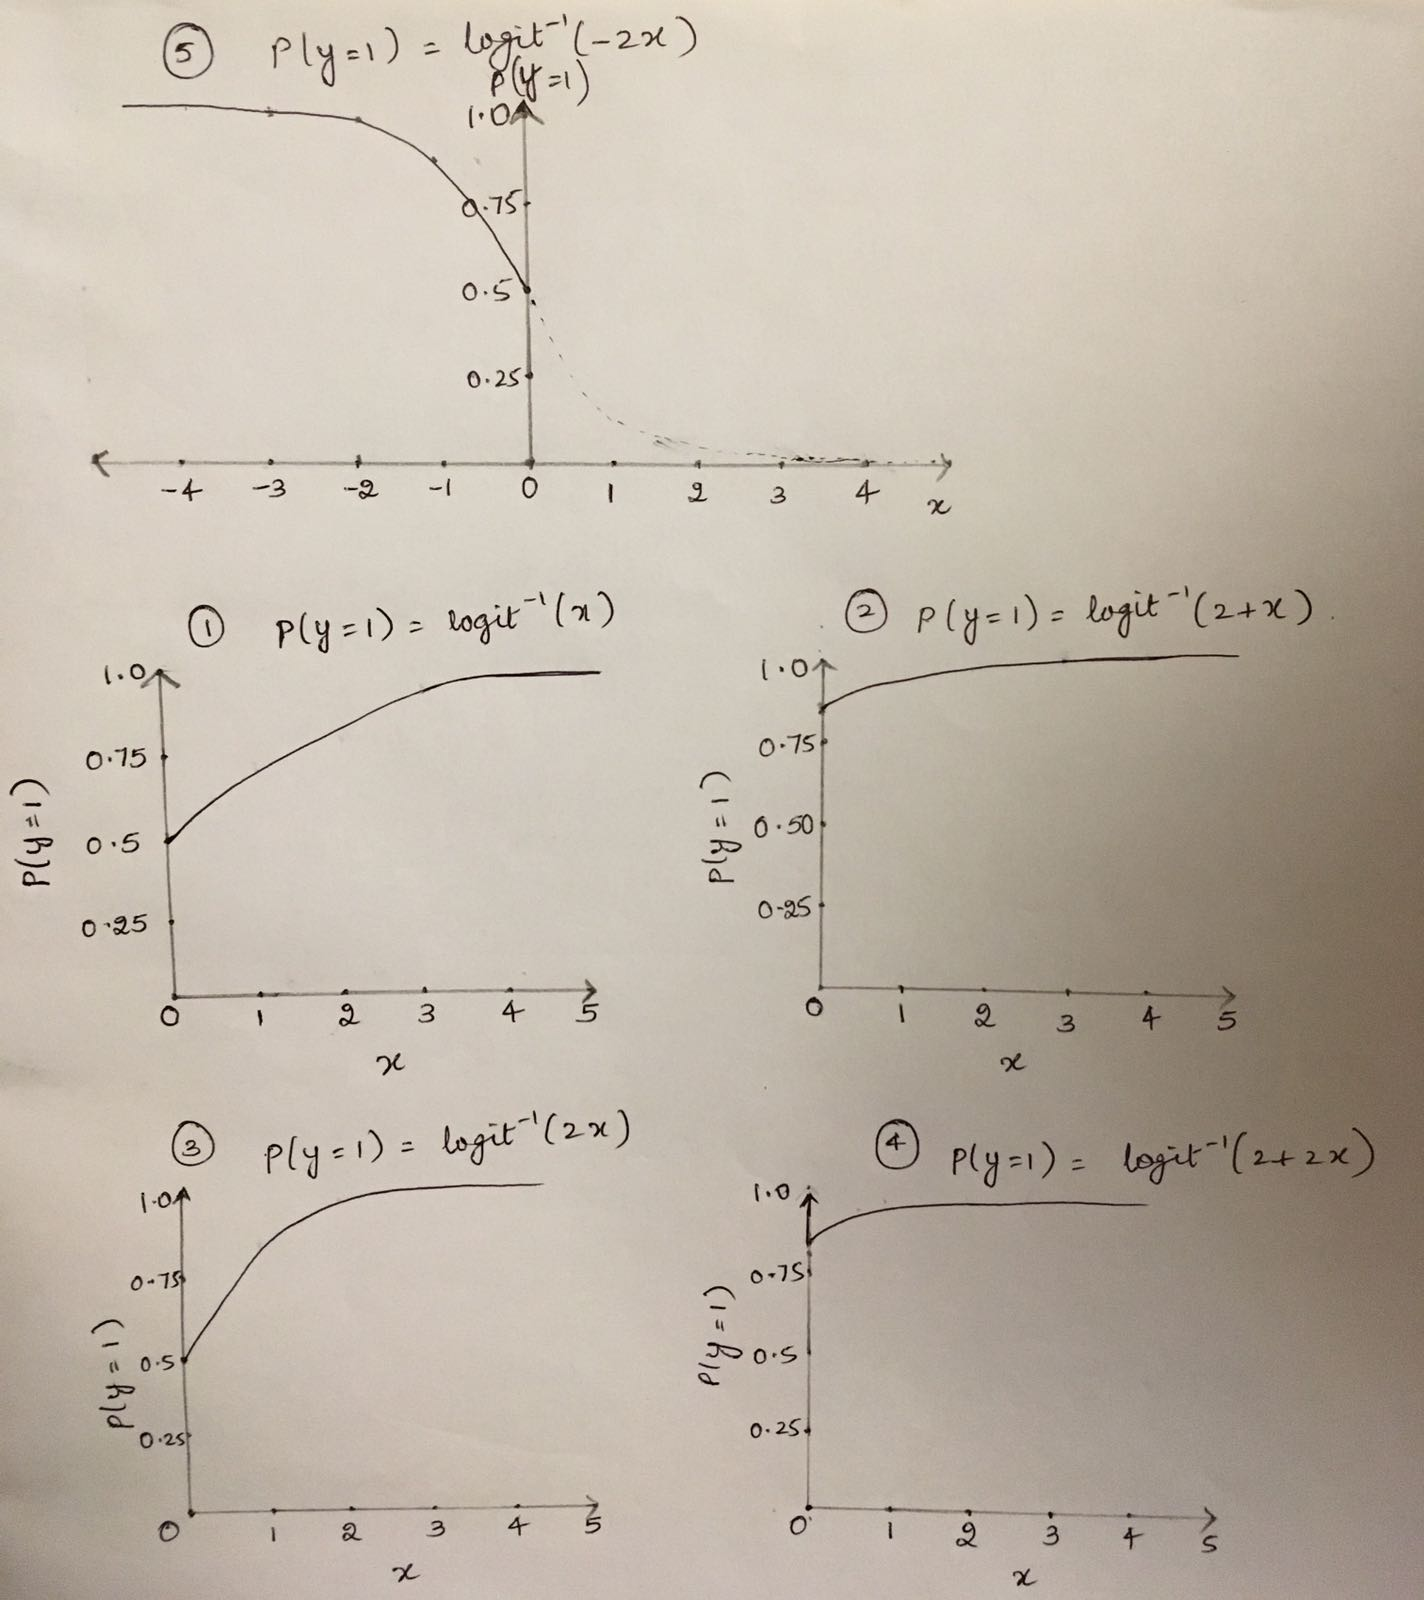
\includegraphics{C:/Users/GP/Desktop/MEGHA/Appl Stat Modelling/Homework/MA678/Homework3} \end{center}

\subsubsection{}\label{section}

In a class of 50 students, a logistic regression is performed of course
grade (pass or fail) on midterm exam score (continuous values with mean
60 and standard deviation 15). The fitted model is
\(Pr(pass) = logit^{-1}(-24+0.4x)\).

\begin{enumerate}
\def\labelenumi{\arabic{enumi}.}
\item
  Graph the fitted model. Also on this graph put a scatterplot of
  hypothetical data consistent with the information given.
\item
  Suppose the midterm scores were transformed to have a mean of 0 and
  standard deviation of 1. What would be the equation of the logistic
  regression using these transformed scores as a predictor?
\item
  Create a new predictor that is pure noise (for example, in R you can
  create \texttt{newpred\ \textless{}-\ rnorm\ (n,0,1)}). Add it to your
  model. How much does the deviance decrease?
\end{enumerate}

\subsubsection{Logistic regression}\label{logistic-regression}

You are interested in how well the combined earnings of the parents in a
child's family predicts high school graduation. You are told that the
probability a child graduates from high school is 27\% for children
whose parents earn no income and is 88\% for children whose parents earn
\$60,000. Determine the logistic regression model that is consistent
with this information. (For simplicity you may want to assume that
income is measured in units of \$10,000).

\subsubsection{Latent-data formulation of the logistic
model:}\label{latent-data-formulation-of-the-logistic-model}

take the model \(Pr(y = 1) = logit^{-1}(1 + 2x_1 + 3x_2)\) and consider
a person for whom \(x_1 = 1\) and \(x_2 = 0.5\). Sketch the distribution
of the latent data for this person. Figure out the probability that
\(y=1\) for the person and shade the corresponding area on your graph.

\subsubsection{Limitations of logistic
regression:}\label{limitations-of-logistic-regression}

consider a dataset with \(n = 20\) points, a single predictor x that
takes on the values \(1, \dots , 20\), and binary data \(y\). Construct
data values \(y_{1}, \dots, y_{20}\) that are inconsistent with any
logistic regression on \(x\). Fit a logistic regression to these data,
plot the data and fitted curve, and explain why you can say that the
model does not fit the data.

\subsubsection{Identifiability:}\label{identifiability}

the folder nes has data from the National Election Studies that were
used in Section 5.1 of the Gelman and Hill to model vote preferences
given income. When we try to fit a similar model using ethnicity as a
predictor, we run into a problem. Here are fits from 1960, 1964, 1968,
and 1972:

\begin{verbatim}
## glm(formula = vote_rep ~ female + black + income, family = binomial(link = "logit"), 
##     data = nes5200_dt_d, subset = (year == 1960))
##             coef.est coef.se
## (Intercept) -0.16     0.23  
## female       0.24     0.14  
## black       -1.06     0.36  
## income       0.03     0.06  
## ---
##   n = 877, k = 4
##   residual deviance = 1202.6, null deviance = 1215.7 (difference = 13.1)
\end{verbatim}

\begin{verbatim}
## glm(formula = vote_rep ~ female + black + income, family = binomial(link = "logit"), 
##     data = nes5200_dt_d, subset = (year == 1964))
##             coef.est coef.se
## (Intercept)  -1.16     0.22 
## female       -0.08     0.14 
## black       -16.83   420.51 
## income        0.19     0.06 
## ---
##   n = 1062, k = 4
##   residual deviance = 1254.0, null deviance = 1337.7 (difference = 83.7)
\end{verbatim}

\begin{verbatim}
## glm(formula = vote_rep ~ female + black + income, family = binomial(link = "logit"), 
##     data = nes5200_dt_d, subset = (year == 1968))
##             coef.est coef.se
## (Intercept)  0.48     0.24  
## female      -0.03     0.15  
## black       -3.64     0.59  
## income      -0.03     0.07  
## ---
##   n = 851, k = 4
##   residual deviance = 1066.8, null deviance = 1173.8 (difference = 107.0)
\end{verbatim}

\begin{verbatim}
## glm(formula = vote_rep ~ female + black + income, family = binomial(link = "logit"), 
##     data = nes5200_dt_d, subset = (year == 1972))
##             coef.est coef.se
## (Intercept)  0.70     0.18  
## female      -0.25     0.12  
## black       -2.58     0.26  
## income       0.08     0.05  
## ---
##   n = 1518, k = 4
##   residual deviance = 1808.3, null deviance = 1973.8 (difference = 165.5)
\end{verbatim}

What happened with the coefficient of black in 1964? Take a look at the
data and figure out where this extreme estimate came from. What can be
done to fit the model in 1964?

\section{Feedback comments etc.}\label{feedback-comments-etc.}

If you have any comments about the homework, or the class, please write
your feedback here. We love to hear your opinions.


\end{document}
